\documentclass[pdftex,english,oribibl]{llncs}

%% Spracheinstellungen laden
\usepackage[english]{babel}

%% Schriftart in der Ausgabe/Eingabe
\usepackage[T1]{fontenc}
\usepackage{textcomp}
\usepackage[latin1]{inputenc}
\usepackage{comment}
%% Zitate
\usepackage[numbers]{natbib}
\bibliographystyle{abbrvnat}
%\bibliographystyle{dinat}
%\bibliographystyle{plainnat}
%\bibliographystyle{splncs}
%% Similar to option "sectionbib" but \refname instead of \bibname
\makeatletter
\renewcommand\bibsection{\section*{\refname\@mkboth{\MakeUppercase{\refname}}{\MakeUppercase{\refname}}}}
\makeatother

%% Index
%\usepackage{makeidx}
%\makeindex

%% PDF Einstellungen
% muss nach natbib geladen werden!
\usepackage{nameref}
\usepackage{varioref}
\usepackage[pdfusetitle,pdftex,colorlinks]{hyperref}
\hypersetup{pdfborder={0 0 0}}
\hypersetup{bookmarksdepth=3}
\hypersetup{bookmarksopen=true}
\hypersetup{bookmarksopenlevel=1}
\hypersetup{bookmarksnumbered=true}
\usepackage{color}
\hypersetup{colorlinks=false}

%\usepackage[section]{tocbibind}

\makeatletter
\gdef\@keywords{}
\def\keywords#1{\gdef\@keywords{#1}}
\gdef\@subtitle{}
\def\subtitle#1{\gdef\@subtitle{#1}}

%% modified from llncs
\renewenvironment{abstract}{%
  \list{}{\advance\topsep by0.35cm\relax\small%
          \leftmargin=1cm%
          \labelwidth=\z@%
          \listparindent=\z@%
          \itemindent\listparindent%
          \rightmargin\leftmargin}%
          \item[\hskip\labelsep\bfseries\abstractname]}{%
  \if!\@keywords!\else{\item[~]\item[\hskip\labelsep\bfseries\keywordname]\@keywords}\fi%
  \endlist}

\AtBeginDocument{%
  \if!\@subtitle!\else\hypersetup{pdfsubject={\@subtitle}}\fi
  \if!\@keywords!\else\hypersetup{pdfkeywords={\@keywords}}\fi
}
\makeatother

% llncs hyperref fix
\makeatletter
\providecommand*{\toclevel@author}{0}
\providecommand*{\toclevel@title}{0}
\makeatother

%% Grafiken
\usepackage[pdftex]{graphicx}
\DeclareGraphicsExtensions{.pdf,.jpg,.png}
\usepackage{subfigure}

%% Mathe
\usepackage{amsmath}
\usepackage{amssymb}

%% Listings
\usepackage{listings}
\lstset{escapechar=\%, frame=tb, basicstyle=\footnotesize}

%% Sonstiges
\newcommand{\TODO}[1]{\par\textcolor{red}{#1}\marginpar{\textcolor{red}{TODO}}}
\newcommand{\TODOX}[1]{\textcolor{red}{#1}\marginpar{\textcolor{red}{TODO}}}
\pagestyle{plain}

% Keine "Schusterjungen"
\clubpenalty = 10000
% Keine "Hurenkinder"
\widowpenalty = 10000 \displaywidowpenalty = 10000

%%%%%%%%%%%%%%%%%%%%%%%%%%%%%%%%%%%%%%%%%%%%%%%%%%%%%%%%%%%%%%%%%%%%%%%%%%%%%%%
%%% BEGIN DOCUMENT
%%%%%%%%%%%%%%%%%%%%%%%%%%%%%%%%%%%%%%%%%%%%%%%%%%%%%%%%%%%%%%%%%%%%%%%%%%%%%%%
\title{Evaluation of Data Quality Assessment}
% \subtitle{My (optional) Subtitle}
\author{KUANG-YU LI}
\institute{University of Stuttgart\\Master Student in Information Technology \\70569 Stuttgart, Germany}


\begin{document}

\maketitle

\begin{abstract}
   The paper provides an evaluation of fives modern data quality (DQ) assessment methods. Due to the diversity and complexity of these assessment methods, fundamentals regarding data quality and classification for assessment method are first presented. With the extension of DQ fundamentals, the paper then reviews five data quality assessment methods and evaluates them in terms of their capability of targeted data types, steps, phases, strategies, techniques, targeted data quality dimensions and cost. The goal of this article is to propose a practical methods in combination of existing methods for data quality assessment  in the context of  continuous integration (CI) and  continuous delivery (CD) application in the field of software engineering. The paper concludes with a suitable method proposal based on the evaluation result and discusses future work and challenges.

\end{abstract}
\section{Introduction}
With the Machine Learning, Deep Learning and Artificial Intelligence on the rise, the demand of data analysis has never been higher.
Both academy and industry sectors are eager to explore more opportunity by employing these techniques.
However, another issue quickly arises: How does one acquire high-quality data? Or, more preciosity, how to defines the quality of a set of data?
There is a famous saying in the field Machine Learning: "Garbage input equals garbage output!".
That is, only with systematic method to assess data set, are ML application feasible for different domain.
Traditionally, data labeling and assessment are done in either primitive or laborious manner, which becomes almost impossible in the big data era.
The goal of this paper is to give an overview of methods to assess data quality and review the most popular data properties that can be analyzed.
Moreover, this paper reviews several proposed data quality improvement methods after data quality is assessed.
The application of the assessment methods are also presented.

The rest of the paper is structured as follows: Data Quality Fundamentals, Literature Review, Evaluation and Conclusion.
For the first section, the overview of data quality and classification of assessment methods are presented,
which includes data type, data problem, phases and steps, strategies and techniques, dimensions and cost.
In second section, literature review of five data quality assessment method, phases and concepts are introduced in brief.
In the third part, evaluation on these five methods is performed in terms of data quality fundamental attributes of previous section .
In the end of paper, a conclusion is made based on evaluation result in the context of CI/CD application in software engineering.
The proposed method, future work and challenges are discussed in brief.
This paper is requested and written under the subtopic of seminar, Advanced Software Engineering:Non-Functional Aspects in Software Engineering.

Main references are base on following paper and journal: \citet{Cai2005ChallnegesOfDataQuality}, \citet{Pipino2002DataQualityAssessment} and \citet{Batini2009MethodologiesForDataQuality} \citet{Wang1996BeyondAccuracy} \citet{Borek2011AClassficationOfDataQualityAssessmentMethods}
   \citet{Cappiello2004DataQualityAssessmentfromTheUse}


\section{Data Quality Fundamentals}
In this section, fundamentals of data and classifications of assessment methods are introduced.
First, in data fundamentals, concepts ans definition of the data type, data quality problem and data quality dimensions are presented. Secondly, in classifications assessment methods, the paper discussed the most common process, pipelines for analysing DQ are introduced.
This topics regarding these methodologies includes steps and phases, strategies and techniques, dimensions, costs.

\subsection{Data Types}
The ultimate goal of a DQ methodology is the analysis of data.
The real world objects need to be created in a format that could further be stored, retrieved and processed by software programs.
In the field of data and computer science, data are either implicitly or explicitly distinguished by three types:

- Structured data, is aggregations or generalizations of items described by elementary attributes defined within a domain.
Domains represent the range of values that can be assigned to attributes and usually correspond to elementary data types of programming languages, such as numeric values or text strings.
Relational tables and statistical data represent the most common type of structured data.

- Unstructured data, is a generic sequence of symbols, typically coded in natural language.
Typical examples of unstructured data are a questionnaire containing free text answering open questions or the body of an e-mail.

- Semistructured data, is data that have a structure which has some degree of flexibility. Semistructured data are also referred to as schemaless or self-describing.
For example, XML, a the markup language commonly used to represent semistructured data, is semistructured.
\begin{comment}
Some common characteristics are:
(1) data can contain fields not known at design time; for instance, an XML file does not have an associated XML schema file;
(2) the same kind of data may be represented in multiple ways; for example, a date might be represented by one field or by multiple fields, even within a single data set; and
(3) among the fields known at design time, many fields will not have values.
\end{comment}

  \begin{figure}
    \centering
    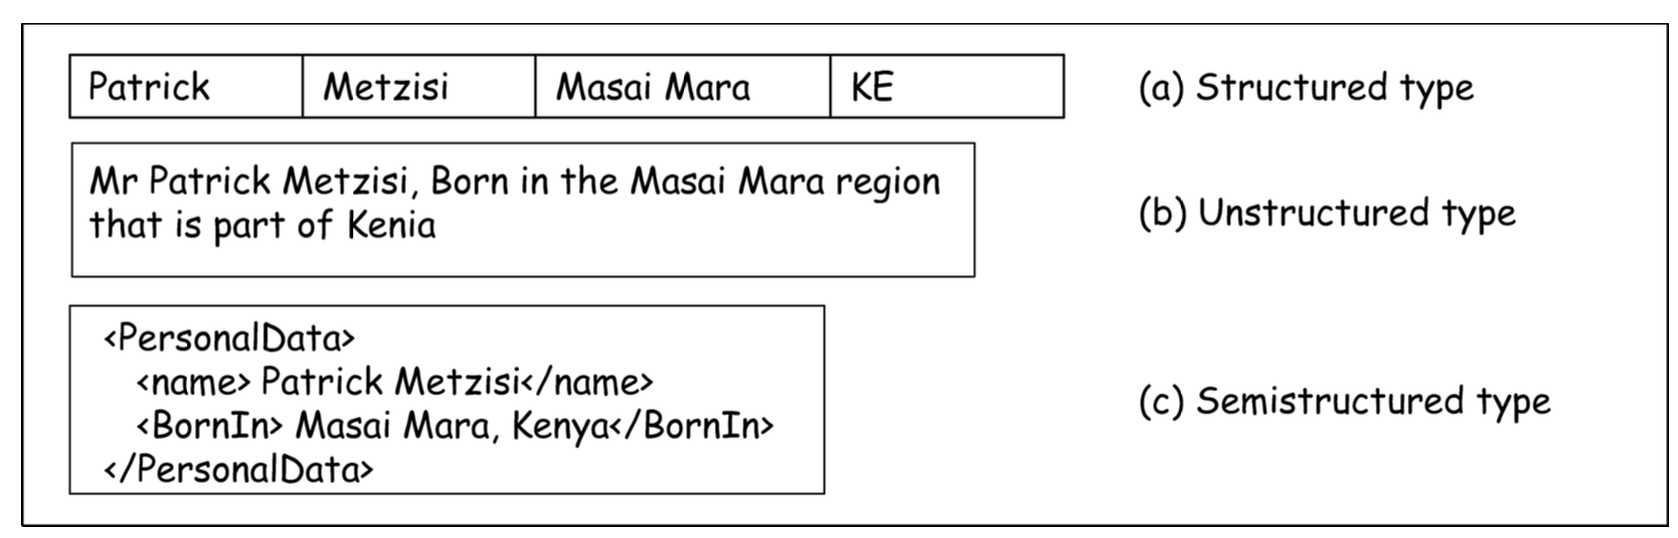
\includegraphics[width=1\textwidth]{Paper/figures/DataType.png}
    \caption{Data Type.}
    \label{fig:datatype}
  \end{figure}

 Data quality techniques become increasingly complex as data lose structure. For example, let us consider a registry describing personal information such as Name, Surname, Region, and StateOfBirth. Figure \ref{fig:datatype} shows the representation of Mr. Patrick Metzisi, born in the Masai Mara region in Kenya, by using a structured Figure \ref{fig:datatype}(a), unstructured (Figure \ref{fig:datatype}(b)), and semistructured (Figure \ref{fig:datatype}(c)) type of data.
 The same quality dimension will have different metrics according to the type of data. This would be explained in later subsection.
 The large majority of research contributions in the data quality literature focuses on structured and semistructured data. For this reason, this report focuses on structured and semistructured data.

\subsection{Data Quality Problems}\label{sec:DataQualityProblems}
The data quality problem could be classified into four categories depending on two factor: context-independence and role perspective.
 Table \ref{table:DataQualityProblem} provides a brief definition for each DQ problem.
 In the context independent category, spelling errors, missing data, and incorrect values are self-explanatory DQ problems.
 Duplicate data problems occur when rows are duplicated or when schemas contain redundancies.
 Data format problems occur when two or more semantically equivalent data values have different representations, including inconsistent and text formatting.
 Syntax violation problems occur when a pre-specified format has been assigned to an attribute and a data value for this attribute does not adhere to this format, including incomplete data format.
 Problems with violations of integrity constraints arise when data values do not adhere to pre-specified database integrity constraints; we also therefore include unique value violations, rather than have these as a separate problem, because unique value violations are one type of database integrity constraint.
 Note that, despite its position in Table we treat outdated data to be a user perspective problem because whether data is out of date depends on the purpose it is used for.

 For the context dependent category, the problem of violation of domain constraints is when an attribute value must be in a pre-specified context-dependent domain of values.
 Violation of organizational business rules is when any set of values do not adhere to a pre-specified rules assigned by the organization.
 Violation of company and governmental regulations is when any set of values do not adhere to a prespecified rules assigned imposed on the organization by legislating bodies.
 Similarly, violation of constraints provided by the database administrator is when any set of values do not adhere to a pre-specified rules assigned by the database administrator. In \ref{sec:DataQualityDimensions}, the problems are define in different dimensions with specific indicators.

 % Please add the following required packages to your document preamble:
% \usepackage[normalem]{ulem}
% \useunder{\uline}{\ul}{}
\begin{table}[]
\begin{tabular}{l|l|l|}
\cline{2-3}
                                                                                     & Data Perspective                                                                                                                                                                                                                                                             & User Perspective                                                                                                                                                                                                                                                                                                                                                                \\ \hline
\multicolumn{1}{|l|}{\begin{tabular}[c]{@{}l@{}}Context-\\ independent\end{tabular}} & \begin{tabular}[c]{@{}l@{}}Spelling error\\ Missing data\\ Duplicate data\\ Incorrect value\\ Inconsistent data format Outdated data\\ Incomplete data format\\ Syntax violation\\ Unique value violation Violation of \\ integrity constraints Text formatting\end{tabular} & \begin{tabular}[c]{@{}l@{}}The information is inaccessible\\ The information is insecure\\ The information is hardly retrievable \\ The information is difficult to aggregate\\ Errors in the information transformation\end{tabular}                                                                                                                                           \\ \hline
\multicolumn{1}{|l|}{\begin{tabular}[c]{@{}l@{}}Context-\\ dependent\end{tabular}}   & \begin{tabular}[c]{@{}l@{}}Violation of domain constraints \\ Violation of organization’s business rules\\ Violation of company and government\\ regulations \\ Violation of constraints provided by\\  the database administrator\end{tabular}                              & \begin{tabular}[c]{@{}l@{}}The information is not based on fact \\ The information is of doubtful credibility\\ The information presents an impartial view\\ The information is irrelevant to the work\\ The information is incomplete\\ The information is compactly represented\\ The information is hard to manipulate \\ The information is hard to understand\end{tabular} \\ \hline
\end{tabular}
\caption{Types of Data Quality Problem}
\label{table:DataQualityProblem}
\end{table}

\subsection{Phases and Steps}
In the most general case, the sequence of activities of a data quality methodology is composed of three phases:
(1) State reconstruction, which is aimed at collecting contextual information on organizational processes and services, data collections and related management procedures, quality issues and corresponding costs; this phase can be skipped if contextual information is available from previous analyses.
(2) Assessment, which measures the quality of data collections along relevant quality dimensions; the term measurement is used to address the issue of measuring the value of a set of data quality dimensions.
\begin{comment}
The term assessment is used when such measurements are compared to reference values, in order to enable a diagnosis of quality. The term assessment is adopted in this article, consistent with the majority of methodologies, which stress the importance of the causes of poor data quality.
\end{comment}
(3) Improvement concerns the selection of the steps, strategies, and techniques for reaching new data quality targets.

\subsubsection{Assessment Steps}
includes:
(1) Data Analysis, which examines data schemas and performs interviews to reach a complete understanding of data and related architectural and management rules;
(2) DQ Requirements Analysis, which surveys the opinion of data users and administrators to identify quality issues and set new quality targets;
(3) Identification of Critical Areas, which selects the most relevant databases and data flows to be assessed quantitatively;
(4) Process Modeling, which provides a model of the processes producing or updating data;
(5) Measurement of Quality, which selects the quality dimensions affected by the quality issues identified in the DQ requirements analysis step and defines corresponding metrics.
\begin{comment}
measurement can be objective when it is based on quantitative metrics, or subjective, when it is based on qualitative evaluations by data administrators and users.
\end{comment}

\subsubsection{Improvement Steps}
includes:
(1) Evaluation of Costs, which estimates the direct and indirect costs of data quality;
(2) Assignment of Process responsibilities, which identifies the process owners and defines their responsibilities on data production and management activities;
(3) Assignment of Data Responsibilities, which identifies the data owners and defines their data management responsibilities;
(4) Identification of the Causes of Errors, which identifies the causes of quality problems;
(5) Selection of Strategies and Techniques, which identifies all the data improvement strategies and corresponding techniques, that comply with contextual knowledge, quality objectives, and budget constraints;
(6) Design of Data Improvement Solutions;
(7) Process Control;
(8) Process Redesign;
(9) Improvement Management;
(10) Improvement Monitoring;

\begin{comment}
(6) Design of Data Improvement Solutions, which selects the most effective and efficient strategy and related set of techniques and tools to improve data quality;
(7) Process Control, which defines check points in the data production processes, to monitor quality during process execution;
(8) Process Redesign, which defines the process improvement actions that can deliver corresponding DQ improvements;
(9) Improvement Management, which defines new organizational rules for data quality;
(10) Improvement Monitoring, which establishes periodic monitoring activities that provide feedback on the results of the improvement process and enables its dynamic tuning.
\end{comment}
Note that in all the steps of the assessment phase, a relevant role is played by metadata that store complementary information on data for a variety of purposes, including data quality. Metadata often provide the information necessary to understand data and/or evaluate them.

\subsection{Strategies and Techniques}
There are two types of strategies: data-driven and process-driven. Data-driven strategies improve the quality of data by directly modifying the value of data and Process-driven strategies improve quality by redesigning the processes that create or modify data.

\subsubsection{Data-Driven Techniques}
includes
(1) Acquisition of New Data, which improves data by acquiring higher-quality data to replace the values that raise quality problems;
(2) Standardization (or Normalization), which replaces or complements nonstandard data values with corresponding values that comply with the standard. For example, nicknames are replaced with corresponding names, for example, Bob with Robert, and abbreviations are replaced with corresponding full names, for example, Channel Str. with Channel Street.
(3) Record Linkage, which identifies that data representations in two (or multiple) tables that might refer to the same real-world object;
(4) Data and Schema Integration, which define a unified view of the data provided by heterogeneous data sources. Integration has the main purpose of allowing a user to access the data stored by heterogeneous data sources through a unified view of these data. Heterogeneities can be classified into technological heterogeneities, schema heterogeneities,and instance-level heterogeneities.
\begin{comment}
In distributed, cooperative, and P2P information systems (see Section 2.6), data sources are characterized by various kinds of heterogeneities that can be generally classified into (1) technological heterogeneities, (2) schema heterogeneities, and (3) instance-level heterogeneities.
Technological heterogeneities are due to the use of products by different vendors, employed at various layers of an information and communication infrastructure.
Schema heterogeneities are primarily caused by the use of (1) different data models, as in the case of a source that adopts the relational data model and a different source that adopts the XML data model, and (2) different representations for the same object, such as two relational sources that represent an object as a table and an attribute. Instance-level heterogeneities are caused by different, conflicting data values provided by distinct sources for the same objects. For instance, this type of heterogeneity can be caused by independent and poorly coordinated processes that feed the different data sources.
Data integration must face all the types of these listed heterogeneities.
\end{comment}
(5) Source Trustworthiness, which selects data sources on the basis of the quality of their data;
(6) Error Localization and Correction, which identify and eliminate data quality errors by detecting the records that do not satisfy a given set of quality rules. These techniques are mainly in the statistical domain.
(7) Cost optimization, defines quality improvement actions along a set of dimensions by minimizing costs.

\subsubsection{Process-Driven Techniques}
- Process control inserts checks and control procedures in the data production process when: (1) new data are created, (2) data sets are updated, or (3) new data sets are accessed by the process. In this way, a reactive strategy is applied to data modification events, thus avoiding data degradation and error propagation.
- Process redesign redesigns processes in order to remove the causes of poor quality and introduces new activities that produce data of higher quality.
\begin{comment}
\subsubsection{Techniques}
 - Column analysis: Number of (unique) values and the number of instances per value as percentage from the total number of instances in that column
 - Cross-domain analysis
 - Data validation
 - Domain analysis
 - Lexical analysis
 - Matching algorithms: identify duplicates
 - Primary key and foreign key analysis (PK/FK analysis) : are good candidates for a PK/FK
 - Schema matching: two attributes are semantically equivalent
 - Semantic profiling
\end{comment}

\subsection{Data Quality Dimensions}\label{sec:DataQualityDimensions}

To define data quality dimension, a data quality is proposed, as shown in Figure \ref{fig:twolayerstandard}. With each dimension, there is underlying data qulity elements and indicators.
In \citet{Cai2005ChallnegesOfDataQuality}, they chose data quality dimensions commonly accepted and widely used as big data quality standards and redefined their basic concepts based on actual business needs.
Each dimension was divided into many typical elements associated with it, and each element has its own corresponding quality indicators: Accessibility
, Timeliness
, Authorization
, Credibility
, Definition/Documentation
, MetaData
, Accuracy
, Consistency
, Integrity
, Completeness
, Auditability
, Fitness
, Readability
,and Structure.
In this way, hierarchical quality standards for big data were used for evaluation.
Figure \ref{fig:twolayerstandard} shows a universal two-layer data quality standard. Detailed correspondence dimension, element and indicators are shown in Figure \ref{fig:hierachicalframwork}.

  \begin{figure}
    \centering
    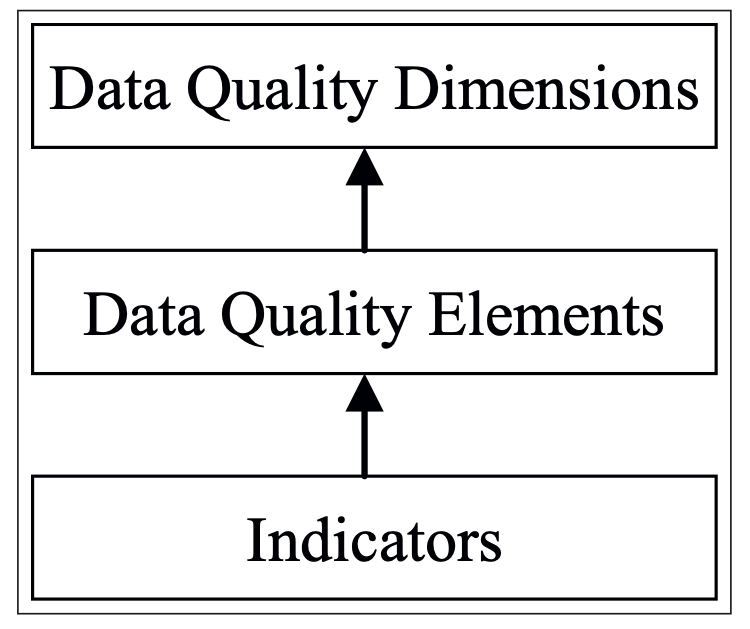
\includegraphics[width=0.25\textwidth]{Paper/figures/DataQualityFramework.png}
    \caption{Data quality framework.}
    \label{fig:dataqualityframework}
  \end{figure}

  \begin{figure}
    \centering
    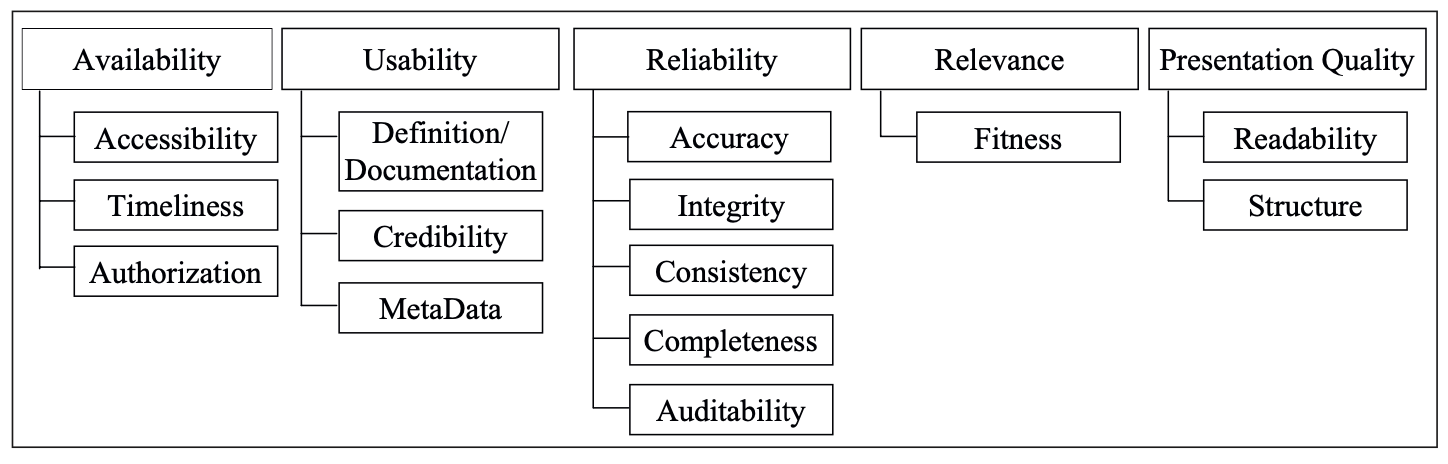
\includegraphics[width=1\textwidth]{Paper/figures/TwoLayerStandard.png}
    \caption{A universal, two-layer big data quality standard for assessment.}
    \label{fig:twolayerstandard}
  \end{figure}

\begin{figure}
    \centering
    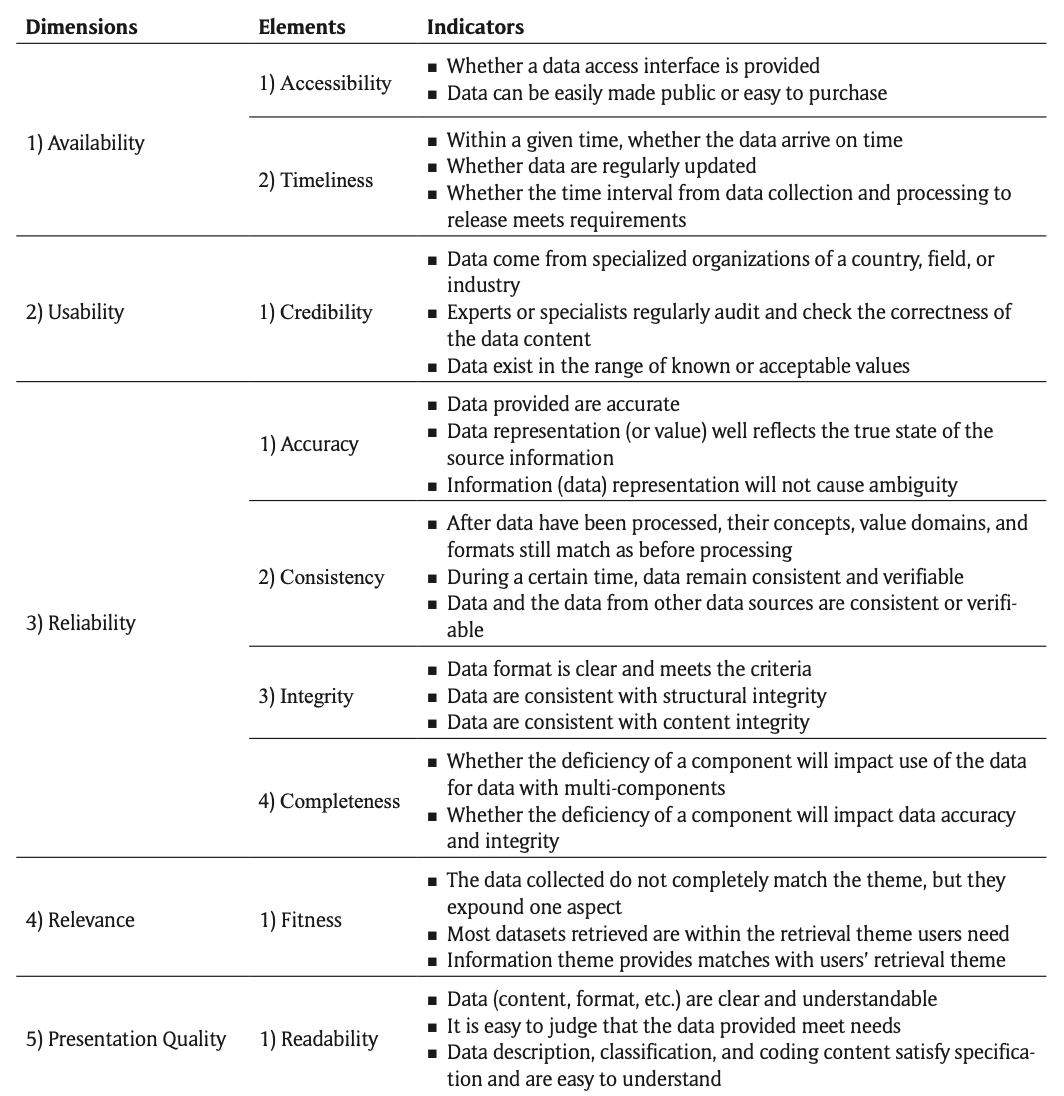
\includegraphics[width=1\textwidth]{Paper/figures/HierarchicalFrameWork.png}
    \caption{The hierarchical big data quality assessment framework(partial content).}
    \label{fig:hierachicalframwork}
 \end{figure}

 For instance, syntactic accuracy is measured as described in Section 2.3 in the case of structured data. With semistructured data, the distance function should consider a global distance related to the shape of the XML tree in addition to the local distance of fields.


\subsection{Cost}
The cost of a data quality program can be considered a preventive cost that is incurred by organizations to reduce data errors. This cost category includes the cost of all phases and steps that compose a data quality assessment and improvement process.
 The costs of poor quality can be classified as:
 (1) process costs, such as the costs associated with the re-execution of the whole process due to data errors;
 (2) opportunity costs due to lost and missed revenues.
 The cost of poor data quality is strongly context-dependent as opposed to the cost of a data quality program. This makes its evaluation particularly difficult, as the same data value and corresponding level of quality has a different impact depending on the recipient. For example, an active trader receiving obsolete information on a stock may incur considerable economic losses as a consequence of wrong investment decisions. In contrast, a newspaper receiving the same obsolete information to publish monthly trading reports may not experience any economic loss.

\section{Literature Review}
In this section, fives data quality assessment methods are introduced in brief, summarizing their characteristics and steps. These methods are Total Data Quality Management (TDQM), Total Information Quality Management (TIQM), Data Quality Assessment (DQA), Information Quality Measurement(IQM), and Comprehensive methodology for Data Quality management(CDQ). The details comparison will be presented in section Evaluation.

\subsection{Total Data Quality Management (TDQM)}\label{sec:TDQM}

The TDQM methodology was the first general methodology published in the data quality literature [Wang 1998]. TDQM is the outcome of academic research, but has been extensively used as a guide to organizational data reengineering initiatives.
Given requirements, reengineering must start from modeling operating processes. Consistent with these tenets, TDQM proposes a language for the description of information production (IP) processes, called IP-MAP [Shankaranarayan et al. 2000]. An information production map is a graphical model designed to help analysts to visualize the information production process, identify the ownership of process phases, understand information and organizational boundaries, and estimate the time and quality metrics associated with the current production process.
The description of processes is a mandatory activity, consistent with the general orientation of process-driven strategies.
\begin{comment}
IP-MAP is the only language for information process modeling and represents a de facto standard. Practical experiences with TDQM are reported, for example, in Kovac and Weickert [2002].
\end{comment}
IP-MAP has been variously extended, towards UML and also to support organizational design.  A example of IP-MAP is shown in Figure \ref{fig:ExampleIPMAP}.

\begin{figure}
    \centering
    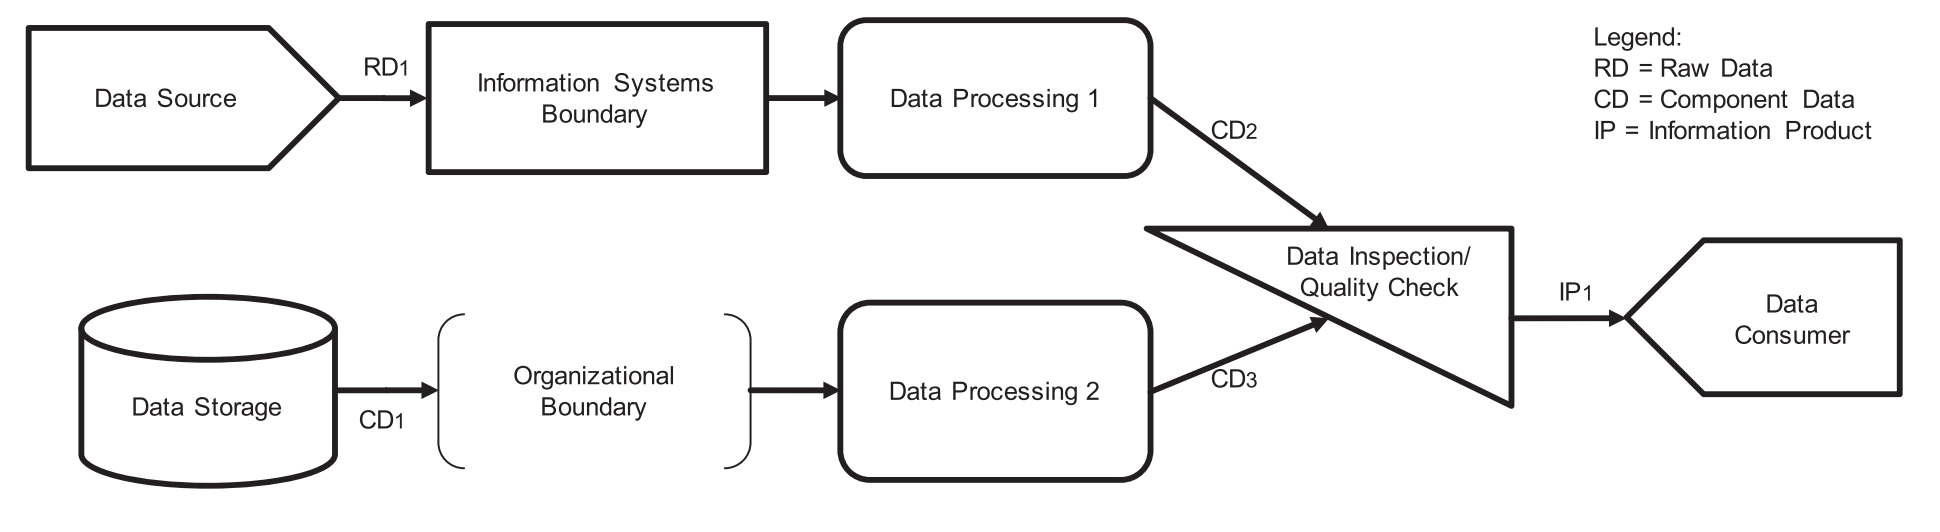
\includegraphics[width=1\textwidth]{Paper/figures/ExampleIPMAP.png}
    \caption{Example of an IP-MAP).}
    \label{fig:ExampleIPMAP}
 \end{figure}


TDQM's goal is to support the entire end-to-end quality improvement process, from requirements analysis to implementation.

As shown in Figure \ref{fig:PhasesTDQM}, TDQM Cycle consists of four phases that implement a continuous quality improvement process: definition, measurement, analysis, and improvement.
The roles responsible for the different phases of the quality improvement process are also defined in TDQM.
Four roles are distinguished: (1) information suppliers, which create or collect data for the IP, (2) information manufacturers, which design, develop, or maintain data and related system infrastructure, (3) information consumers, which use data in their work, and  (4) information process managers, which are responsible for managing the entire information production process throughout the information life cycle.

TDQM relies on the information quality literature for IQ Criteria and IQ improvement techniques and relates quality issues to corresponding improvement techniques.
TDQM is comprehensive also from an implementation perspective, as it provides guidelines as to how to apply the methodology.

\begin{comment}
In applying TDQM, an organization must:
(a) clearly understand the IPs;
(b) establish an IP team consisting of a senior executive as the TDQM champion, an IP engineer who is familiar with the TDQM methodology, and members who are information suppliers, manufacturers, consumers, and IP managers;
(c) teach IQ assessment and IQ management to all the IP constituencies; and
(d) institutionalize continuous IP improvement.
\end{comment}



\begin{figure}
    \centering
    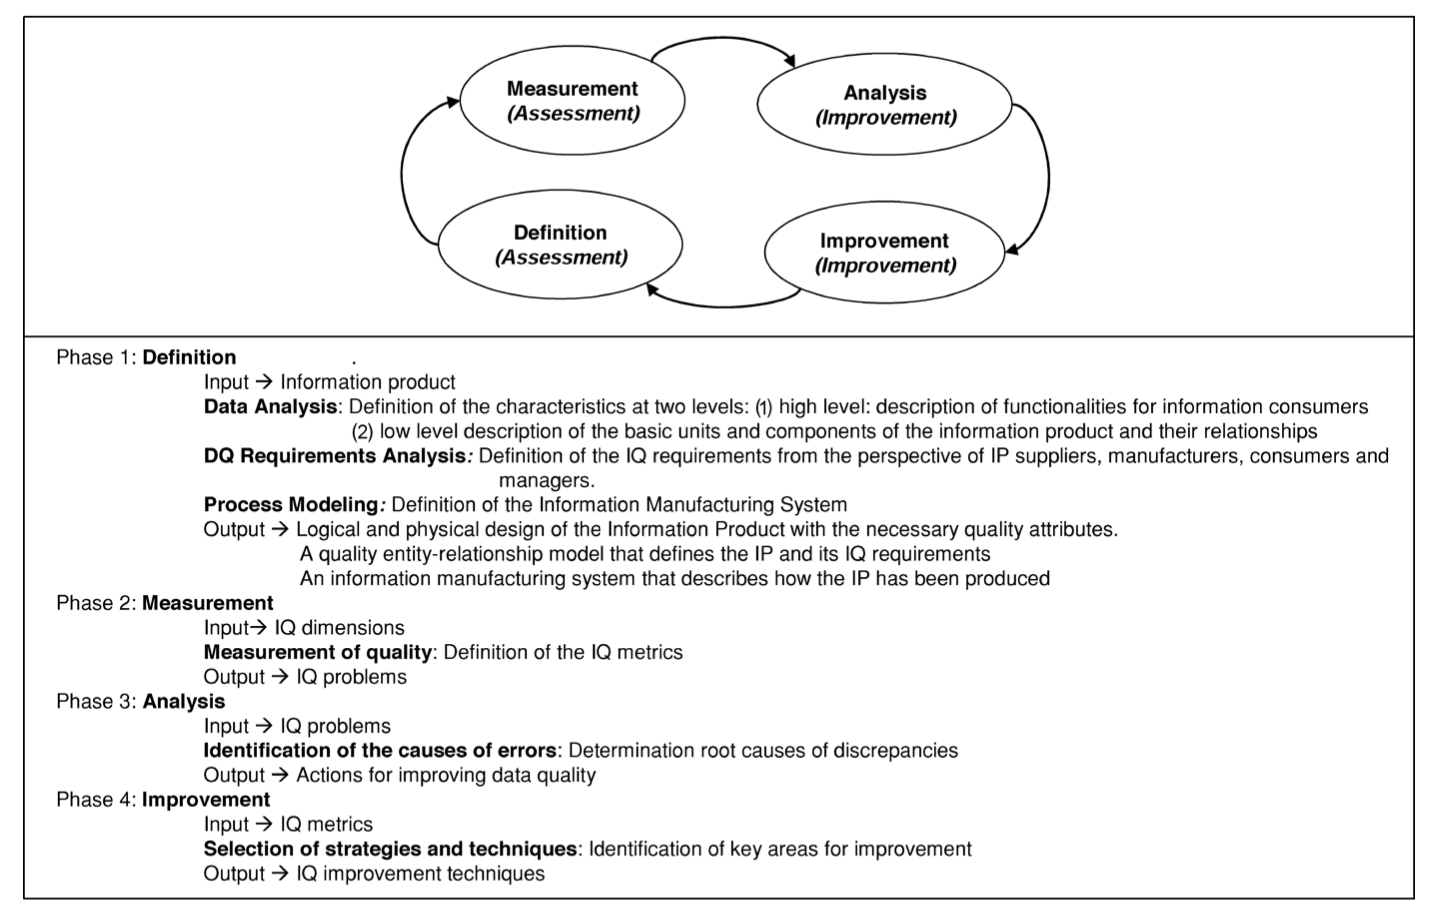
\includegraphics[width=1\textwidth]{Paper/figures/PhasesTDQM.png}
    \caption{TDQM Phases.}
    \label{fig:PhasesTDQM}
 \end{figure}

\subsection{Total Information Quality Management (TIQM)}

The TIQM methodology [English 1999] has been designed to support data warehouse projects. The methodology assumes the consolidation of operational data sources into a unique, integrated database, used in all types of aggregations performed to build the data warehouse. This consolidation eliminates errors and heterogeneities of source databases. TIQM focuses on the management activities that are responsible for the integration of operational data sources, by discussing the strategy that has to be followed by the organization in order to make effective technical choices. Cost-benefit analyses are supported from a managerial perspective. The methodology provides a detailed classification of costs and benefits.

\begin{figure}
    \centering
    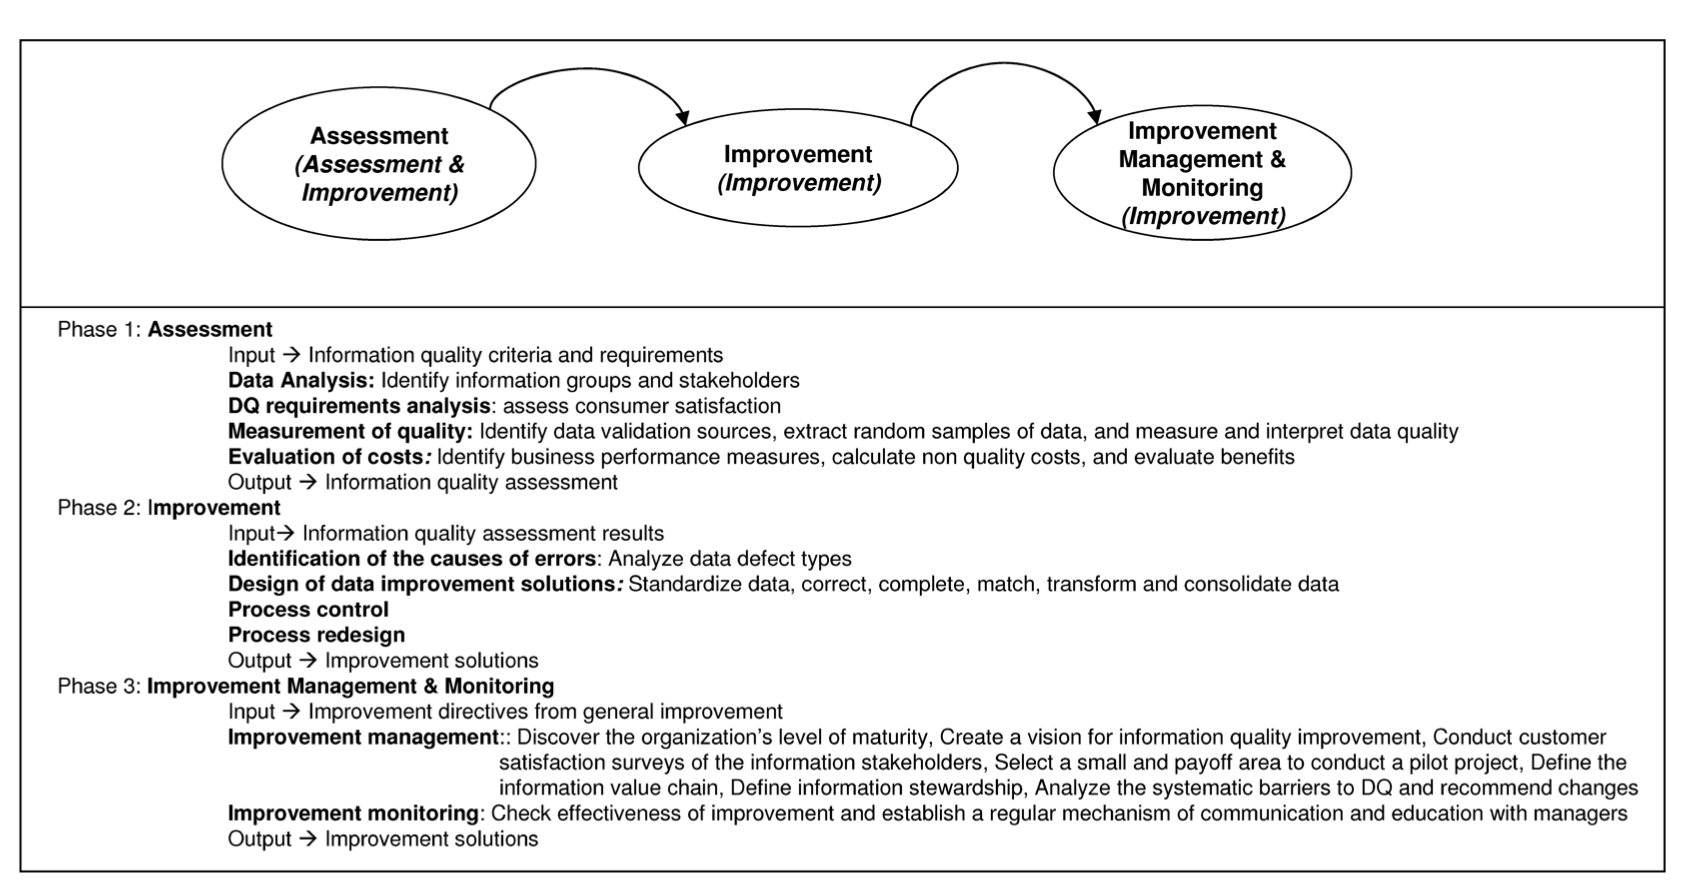
\includegraphics[width=1\textwidth]{Paper/figures/PhasesTIQM.png}
    \caption{TIQM Phases.}
    \label{fig:PhasesTIQM}
 \end{figure}

Figure \ref{fig:PhasesTIQM} shows the phases of the TIQM methodology.
From the TIQM's managerial perspective, there are three main phases: assessment, improvement, and improvement management and monitoring.
One of the valuable contributions of the methodology is the definition of this last phase, which provides guidelines to manage changes in the organization’s structure according to data quality management requirements.
Furthermore, the economics approach introduces cost benefit evaluation to justify data quality interventions.
The goal is not only the achievement of higher data quality level, but to undertake improvement actions only if they are feasible; thus only if benefits are greater than costs.

\subsection{Data Quality Assessment (DQA)}
\begin{figure}
    \centering
    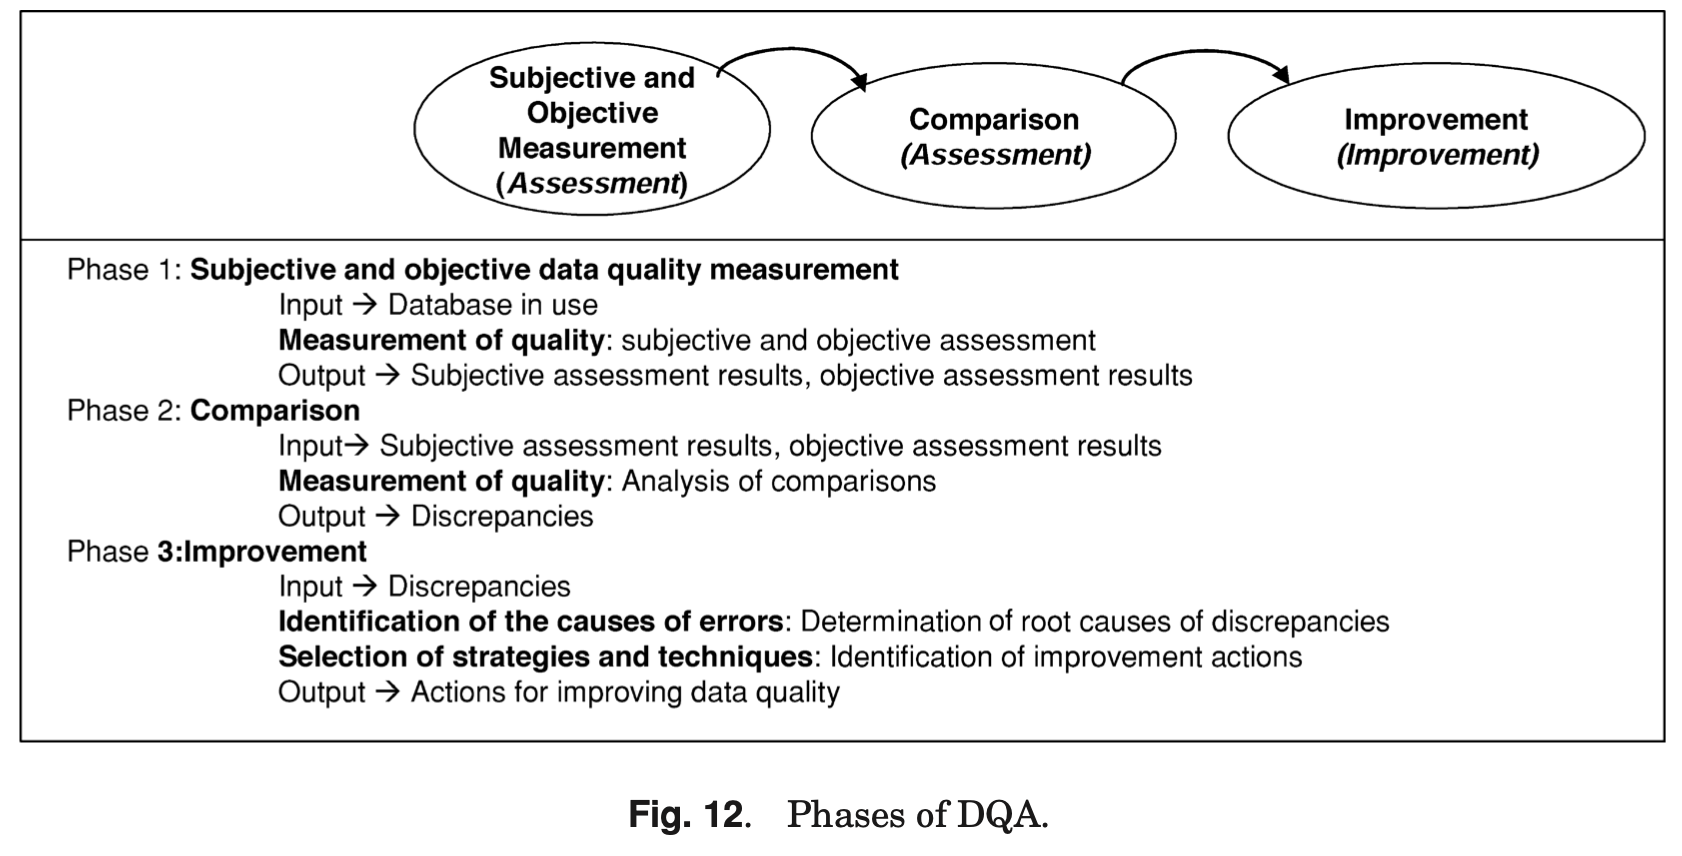
\includegraphics[width=1\textwidth]{Paper/figures/PhasesDQA.png}
    \caption{DQA Phases.}
    \label{fig:PhasesDQA}
 \end{figure}

The DQA methodology [Pipino et al. 2002] has been designed to provide the general principles guiding the definition of data quality metrics. In the literature, data quality metrics are mostly defined ad hoc to solve specific problems and thus, are dependent on the considered scenario. The DQA methodology is aimed at identifying the general quality measurement principles common to previous research. Figure \ref{fig:PhasesDQA} shows the phases.
The methodology makes a distinction between subjective and objective quality metrics. Subjective metrics measure the perceptions, needs, and experiences of the stakeholders. Objective metrics are then classified into task-independent and task-dependent. The first assess the quality of data without contextual knowledge of the application, while the second are defined for specific application contexts and include business rules, company and government regulations, and constraints provided by the database administration. Both metrics are divided into three classes: simple ratio, min or max value, and weighed average.


\subsection{Information Quality Measurement (IQM)}
The fundamental objective of the IQM methodology [Eppler and Mu ̈nzenmaier 2002] is to provide an information quality framework tailored to Web data.
In particular, IQM helps the quality-based selection and personalization of the tools that support Webmasters in creating, managing, and maintaining Web sites.
\begin{figure}
    \centering
    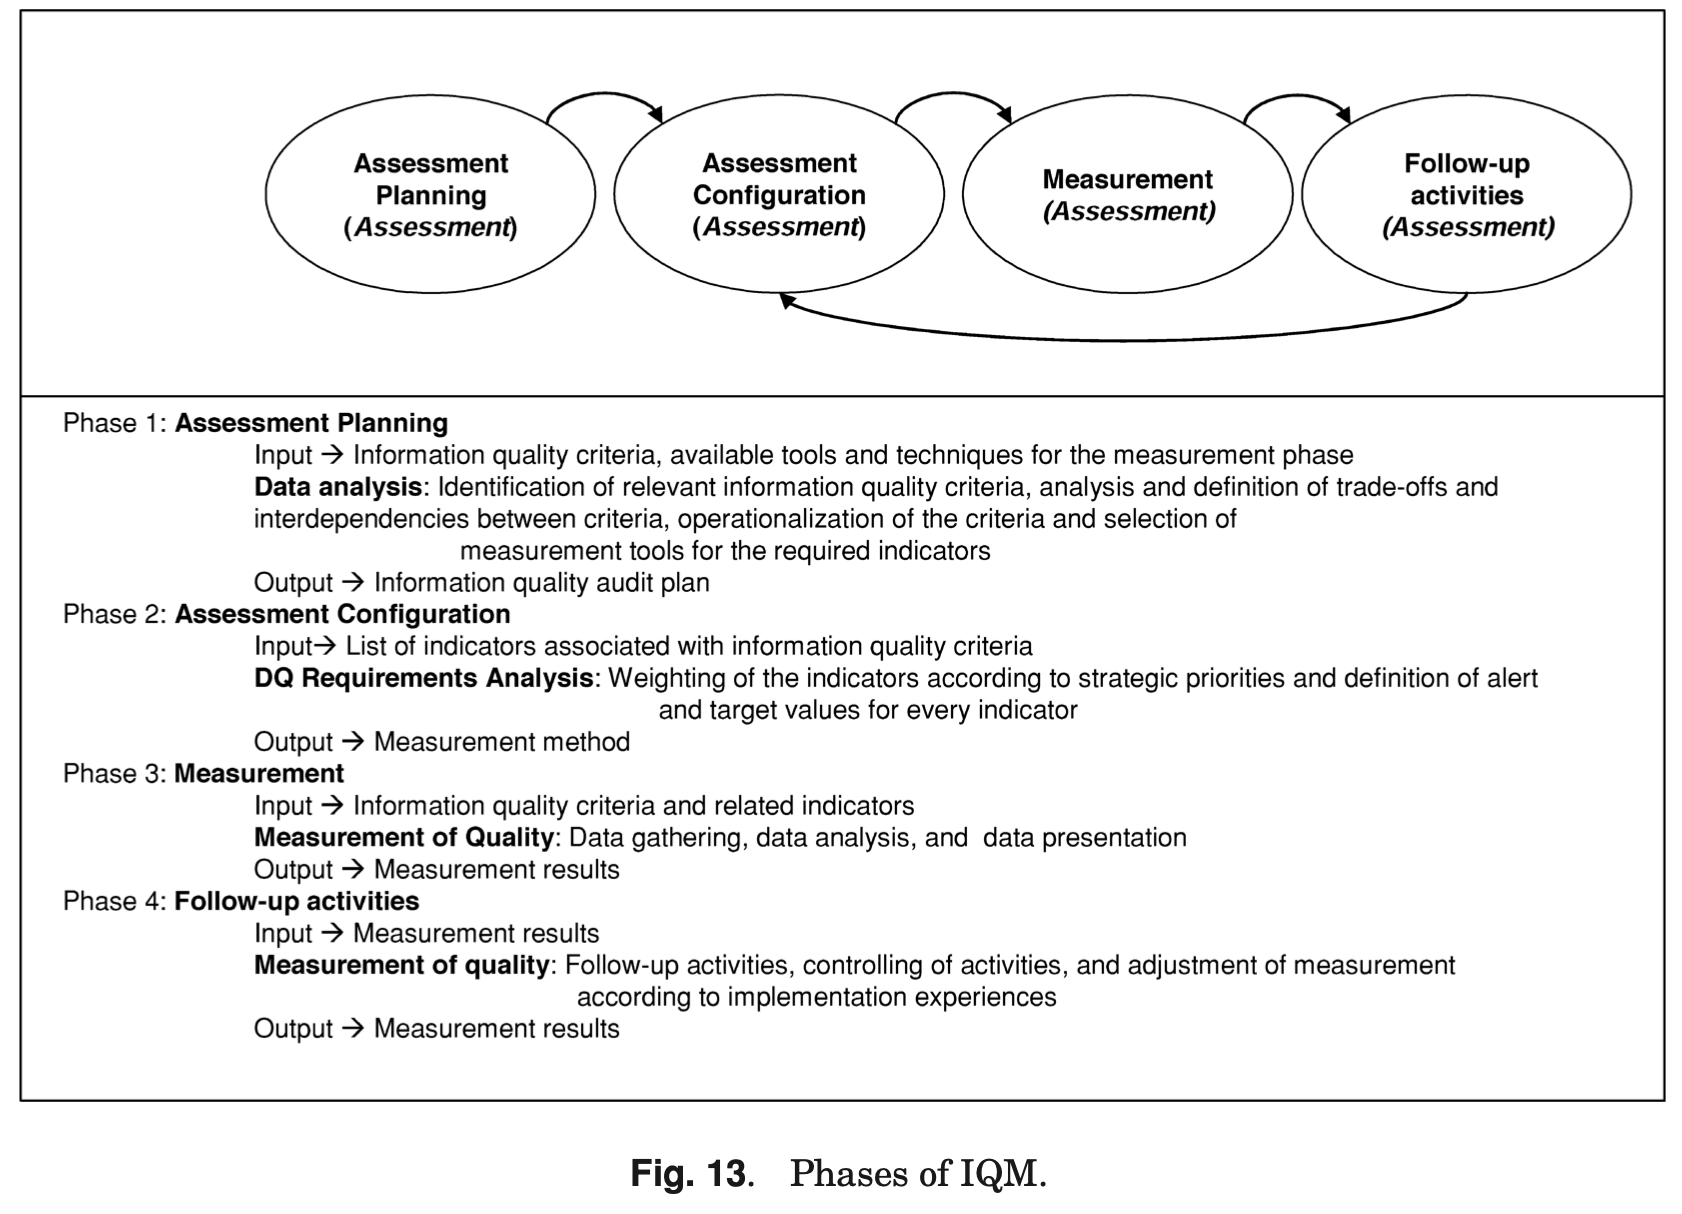
\includegraphics[width=1\textwidth]{Paper/figures/PhasesIQM.png}
    \caption{IQM Phases.}
    \label{fig:PhasesIQM}
 \end{figure}

The IQM methodology provides guidelines to ensure that software tools evaluate all the fundamental information quality dimensions.
The methodology provides two sets of guidelines: the information quality framework defining quality criteria, and the action plan explaining how to perform quality measurements.
The main phases of IQM methodology are reported in \ref{fig:PhasesIQM}. The first phase defines the measurement plan.
The information quality framework is defined as a list of relevant information quality criteria identified by interviewing the information stake- holders.
The framework is the input for an information quality audit that associates the information quality criteria with the methods and tools that will be used in the measurement process.
Some criteria require multiple measurement methods. The IQM methodology coordinates the application of multiple measurement methods.

\subsection{Comprehensive methodology for Data Quality management (CDQ)}

The CDQ methodology [Batini and Scannapieco 2006; Batini et al. 2008] is conceived to be at the same time complete, flexible, and simple to apply.

\begin{comment}
Completeness is achieved by considering existing techniques and tools and integrating them in a framework that can work in both intra- and inter-organizational contexts, and can be applied to all types of data, structured, semistructured and unstructured.
The methodology is flexible since it supports the user in the selection of the most suitable techniques and tools within each phase and in any context.
Finally, CDQ is simple since it is organized in phases and each phase is characterized by a specific goal and set of techniques to apply.

In fact, the other methodologies implicitly assume that contextual knowledge has been previously gathered and modelled.
\end{comment}

The CDQ provides support to select the optimal quality improvement process that maximizes benefits within given budget limits and emphasizes the initial requirements elicitation phase.
The focus is on how to reach total data quality without providing indications as to how to use contextual knowledge. A goal of CDQ is instead to obtain a quantitative assessment of the extent to which business processes are affected by bad information.

\begin{figure}
    \centering
    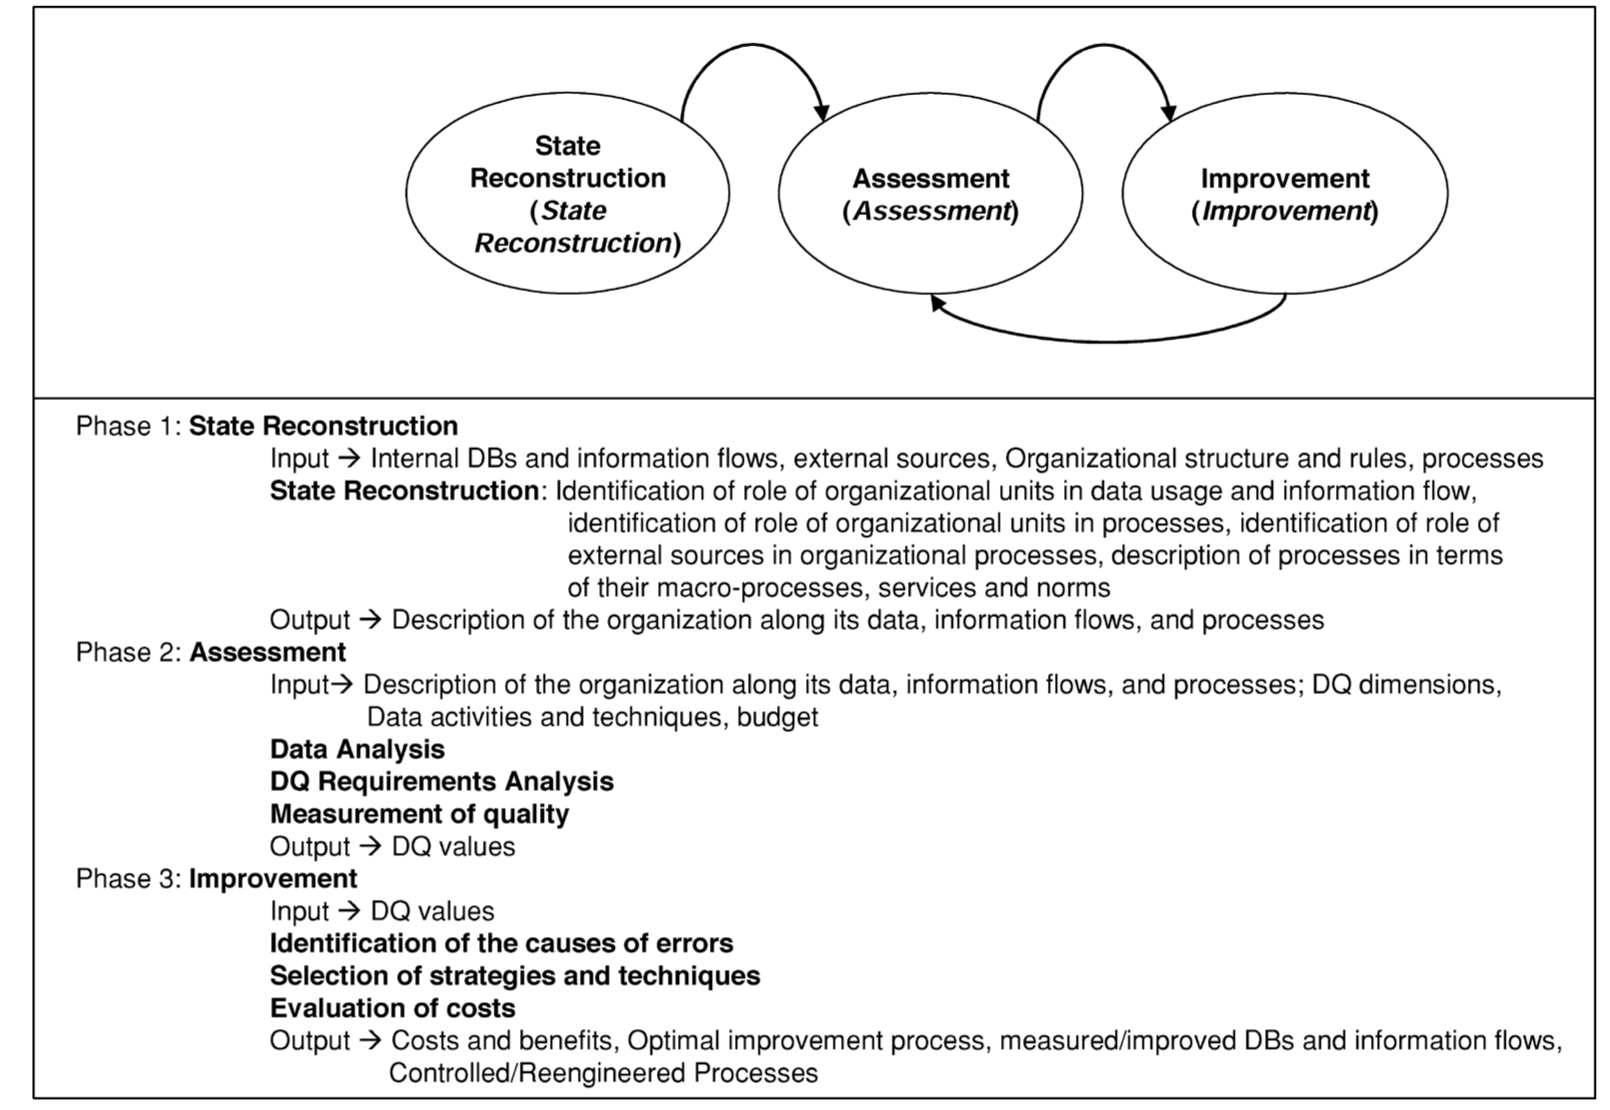
\includegraphics[width=1\textwidth]{Paper/figures/PhasesCDQ.png}
    \caption{CDQ Phases.}
    \label{fig:PhasesCDQ}
 \end{figure}

Three main phases characterize the methodology: state reconstruction, assessment, and choice of the optimal improvement process shown in Figure \ref{fig:PhasesCDQ}.
In the first phase of the methodology, the relationships among organizational units, processes, services, and data are reconstructed.
These relationships are modelled by using matrices that describe which organizational units use data and their roles in the different business processes.
Furthermore, in this phase, processes are described along with their contribution in the production of goods/services and the legal and organizational rules that discipline workflows.
The second phase sets new target quality levels that are needed to improve process qualities, and evaluates corresponding costs and benefits.
This phase locates the critical variables affected by poor quality. Since improvement activities are complex and costly, it is advisable to focus on the parts of the databases and data flows that raise major problems.
Finally, the third phase consists of five steps and is aimed at the identification of the optimal improvement process: the sequence of activities that has the highest cost/effectiveness ratio.
New target quality levels are set by considering costs and benefits. Different improvement activities can be performed to reach new quality targets.
The methodology recommends the identification of all the data-driven and process-driven improvement techniques for the different databases affected by poor quality.
A set of mutually consistent improvement techniques constitutes an improvement process.
Finally, the most suitable improvement process is selected by performing a cost-benefit analysis.


\section{Evaluation}
In this section evaluation in terns of process, techniques, and performances are discussed across these methods.

\subsection{Types of Data}
The supported data types are shown in Table \ref{table:DataTypeComparison}.
It is marked with implicitly considered when the methodology does not explicitly mention the type of data, but phases and steps can be applied to it. CDQ attempts an extension to semistructured data of steps and techniques originally developed for structured data.
\begin{table}[]
\centering
\begin{tabular}{|c|c|c|}
\hline
\begin{tabular}[c]{@{}c@{}}Strategy/Meth. \\ Acronym\end{tabular} & Structured & Semistructured        \\ \hline
TDQM                                                              & x          & x                     \\ \hline
TIQM                                                              & x          & Implicitly considered \\ \hline
DQA                                                               & x          &                       \\ \hline
IQM                                                               & x          & x                     \\ \hline
CDQ                                                               & x          & x                     \\ \hline
\end{tabular}
\caption{Data Type Comparison}
\label{table:DataTypeComparison}
\end{table}


\subsection{Phases and Steps}

\subsubsection{Assessment Phases}
The most commonly addressed steps of the assessment phase are data analysis and measurement of quality. However, they are performed according to different approaches.
Different measurement approaches meet the specific requirements of different organizational contexts, processes, users or services. Only a few methodologies consider the DQ requirements analysis step, identifying DQ issues and collecting new target quality levels from users. This step is particularly relevant for evaluating and solving conflicts in target DQ levels from different stakeholders.
The last column of Table \ref{table:AssessmentStepsComparison} specifies whether the methodology allows extensibility to dimensions (and metrics) other than those explicitly dealt with in the methodology.
CDQ explicitly mentions dimensions, but the approach can be easily generalized to other dimensions.

\begin{table}[]
\begin{tabular}{|c|c|c|c|c|c|c|}
\hline
\begin{tabular}[c]{@{}c@{}}Step/Meth\\ Acronym\end{tabular} & \begin{tabular}[c]{@{}c@{}}Data\\ Analysis\end{tabular} & \begin{tabular}[c]{@{}c@{}}DQ\\ Requirement\\ Analysis\end{tabular} & \begin{tabular}[c]{@{}c@{}}Identification of\\ Critical Areas\end{tabular} & \begin{tabular}[c]{@{}c@{}}Process\\ Modeling\end{tabular} & \begin{tabular}[c]{@{}c@{}}Measurement\\ of Quality\end{tabular} & \begin{tabular}[c]{@{}c@{}}Extensible\\  to Other\\ Dimensions\\ and Metrics\end{tabular} \\ \hline
TDQM                                                        & +                                                       &                                                                     & +                                                                          & +                                                          & +                                                                & Fixed                                                                                     \\ \hline
TIQM                                                        & +                                                       & +                                                                   & +                                                                          & +                                                          & +                                                                & Fixed                                                                                     \\ \hline
DQA                                                         & +                                                       &                                                                     & +                                                                          &                                                            & +                                                                & Open                                                                                      \\ \hline
IQM                                                         & +                                                       &                                                                     &                                                                            &                                                            & +                                                                & Open                                                                                      \\ \hline
CDQ                                                         & +                                                       & +                                                                   & +                                                                          & +                                                          & +                                                                & Open                                                                                      \\ \hline
\end{tabular}
\caption{Assessment Steps Comparison}
\label{table:AssessmentStepsComparison}
\end{table}

\subsubsection{Improvement Phases}
Table \ref{table:ImprovementStepsComparison} compares the steps of improvement phases. Since IQM doesn't have improvement phase, the whole column is left empty.
The identification of the causes of errors is the most widely addressed improvement step.
DQA emphasizes the importance of the identification of the causes of errors step, but it does not discuss its execution.
In contrast, the management of the improvement solution step is explicitly performed only by TDQM.
Other methodologies refer to the broad range of management techniques and best practices.
Furthermore, it is possible to repeat the assessment phase of the methodology in order to evaluate the results of the improvement phase.
As an example, DQA explicitly recommends the application of previous methodological steps to evaluate the effectiveness of improvement.
Finally, the relationship among data quality, process, and organization is considered by TIQM, TDQM, and CDQ.
These methodologies thoroughly discuss the assignment of responsibilities on processes and data.
These steps are supported by the results of the state reconstruction phase.
CDQ discusses a set of matrices to represent the relationship among processes, organizational units, and databases, which are produced during the state reconstruction phase and are subsequently used in the assignment of responsibilities steps.

\begin{table}[]
\centering
\begin{tabular}{|c|c|c|c|c|c|}
\hline
\begin{tabular}[c]{@{}c@{}}Step/Meth Acronym\end{tabular} & TDQM & TIQM & DQA & IQM & CDQ \\ \hline
Evaluation of Costs                                         & +    & +    &     &     & +   \\ \hline
Assignment of Process Responsibilities                      & +    & +    &     &     & +   \\ \hline
Assignment of Data Responsibilities                         & +    & +    &     &     & +   \\ \hline
Selection Strategies and Techniques                         & +    & +    &     &     & +   \\ \hline
Identification the Causes of Errors                         & +    & +    & +   &     & +   \\ \hline
Process Control                                             &      &      &     &     & +   \\ \hline
Design of data Improvement Solutions                        &      & +    &     &     & +   \\ \hline
Process Redesign                                            & +    & +    &     &     & +   \\ \hline
Improvement Management                                      & +    &      &     &     &     \\ \hline
Improvement Monitoring                                      & +    & +    &     &     & +   \\ \hline
\end{tabular}
\caption{Improvement Steps Comparison}
\label{table:ImprovementStepsComparison}
\end{table}

\begin{table}[]
\centering
\begin{tabular}{|l|l|l|}
\hline
Strategy/Meth. Acronym & Data-driven                                                                                                                            & Process-driven   \\ \hline
TDQM                   &                                                                                                                                        & Process Redesign \\ \hline
TIQM                   & \begin{tabular}[c]{@{}l@{}}Data cleansing\\ Normalization\\ Error localization and correction\end{tabular}                             & Process Redesign \\ \hline
CDQ                    & \begin{tabular}[c]{@{}l@{}}Normalization\\ Record Linkage\\ Data and schema integration \\ Error localization and correction\end{tabular} & Process Redesign \\ \hline
\end{tabular}
\caption{Strategy Types Comparison}
\label{table:StrategyTypesComparison}
\end{table}

\subsection{Strategies and Techniques}
Table \ref{table:StrategyTypesComparison} shows the strategies and techniques adopted by different methodologies. A methodology is associated with a strategy if it provides guidelines to select and design corresponding techniques.
Notice that the column labelled Process-driven in Table \ref{table:StrategyTypesComparison} provides the same information as columns, Process control and Process redesign of Table \ref{table:ImprovementStepsComparison}. The column labelled Data-driven explicitly mentions the data-driven techniques implicitly considered in Tables \ref{table:ImprovementStepsComparison}.
Table \ref{table:StrategyTypesComparison} shows that two DQ methodologies adopt mixed strategies, variously combining data-driven and process-driven techniques. The methodology applying the wider range of data- and process-driven techniques is TIQM. Conversely, TDQM provides guidelines to apply process-driven strategies by using the Information Manufacturing Analysis Matrix, which suggests when and how to improve data.
Normalization, record linkage, data and schema integration, represent the data- driven techniques most widely adopted in DQ methodologies, while process redesign, as discussed in previous section, is most relevant in process-driven methodologies. We now discuss specific contributions related to the data- and process-driven techniques considered.

\subsubsection{Data-Driven Techniques}
Normalization techniques have been proposed in several domains, including census and territorial data domains.
CDQ provide normalization techniques improving DQ by comparing data with look-up tables and defining a common metaschema.
Record linkage has been investigated in the database research since the 1950s and has been applied in many contexts such as healthcare, administrative, and census applications.
In such contexts, it is crucial to produce efficient computer-assisted matching procedures that can reduce the use of clerical resources, and at the same time, minimize matching errors.
CDQ discusses three types of record linkage techniques:
(1) Probabilistic techniques, based on the broad set of methods developed over the past two centuries within statistics and probability theory, ranging from Bayesian net- works to data mining.
(2) Empirical techniques that make use of algorithmic techniques such as sorting, tree analysis, neighbor comparison, and pruning.
(3) Knowledge-based techniques, extracting knowledge from files and applying reasoning strategies.
Criteria for choosing among these three types of techniques are discussed within the CDQ methodology.

CDQ emphasizes on the autonomy of organizations in the cooperative system.
In fact, the resolution of heterogeneities in the case studies, proposed as best practices, is performed through record linkage on a very thin layer of data, namely the identifiers.
All other data are reconciled only in case of autonomous decisions of the agencies involved.
\subsubsection{Process-Driven Techniques}
Methodologies addressing the process redesign step tend to borrow corresponding techniques from business process reengineering (BPR).
TDQM represents an exception in this respect, as it proposes an original process redesign control approach that is referred to as an "information manufacturing system for the Information Product".
This methodology proposes the Information Production Map (IP-MAP) model, introduced in Section \ref{sec:TDQM}.
After modelling and assessing the information production process, new process control activities are identified and/or process redesign decisions are taken.

Complex solutions such as IP-MAP cannot always be adopted due to their high costs and, in some cases, the practical unfeasibility of a thorough process modeling step.
For this reason, other methodologies adopt less formal, but more feasible solutions.
For example, CDQ is based on a set of matrices that describe the main relationships among data, information flows, processes, and organizational units.
\begin{comment}
The relationship between organizational units and processes has also been modeled in extensions of IP-MAP proposed in the literature [Scannapieco et al. 2002].
\end{comment}

\subsection{Data Quality Dimensions}
Table \ref{table:SummaryDataQualityDimension} shows the quality dimensions considered by the methodologies surveyed in this article.
In Table \ref{table:SummaryDataQualityDimension}, a dimension is associated with a methodology, if the methodology provides a corresponding definition.
For each methodology’s dimensions, we address the corresponding references.

\begin{table}[]
\centering
\begin{tabular}{|l|l|l|l|l|l|}
\hline
\multicolumn{1}{|c|}{\begin{tabular}[c]{@{}c@{}}Strategy/Meth. \\ Acronym\end{tabular}} & TDQM & TIQM & DQA & IQM & CDQ \\ \hline
Accessibility                                                                           & +    &      & +   & +   &     \\ \hline
Completeness                                                                            & +    & +    & +   &     & +   \\ \hline
Timeliness                                                                              & +    & +    & +   & +   & +   \\ \hline
Consistency                                                                             & +    & +    & +   & +   & +   \\ \hline
Security                                                                                & +    & +    & +   & +   &     \\ \hline
Correctness                                                                             &      &      &     & +   & +   \\ \hline
Cost                                                                                    &      & +    &     &     & +   \\ \hline
Reputation                                                                              & +    & +    & +   &     & +   \\ \hline
Accuracy                                                                                &      & +    &     & +   & +   \\ \hline
Appropriateness                                                                         & +    &      & +   &     &     \\ \hline
Believability                                                                           & +    &      & +   &     &     \\ \hline
Understandability                                                                       & +    & +    & +   &     &     \\ \hline
\end{tabular}
\caption{Summary Data Quality Dimension}
\label{table:SummaryDataQualityDimension}
\end{table}


Notice the large variety of dimensions defined in the methodologies, which confirms the complexity of the data quality concept. This is not surprising, since nowadays a large number of phenomena can be described in terms of data. Multiple classifications of quality dimensions are proposed by the methodologies. TIQM classifies dimensions as inherent and pragmatic.
CDQ proposes schema and data dimensions.
Due to different metrics and corresponding definition used in different methodology, here we will not go into the detail of each metrics. In some methodology, even different metrics are used for the same dimension.

\begin{comment}
Table IX shows the metrics provided for quality dimensions by different methodologies.
We do not include metrics for semantic accuracy because the methodology addressing it, CDQ, do not provide specific measurement methods.
In general, multiple metrics are defined for each dimension, and each dimension accordingly has multiple entries in the table.
Note that subjective metrics such as user surveys have been defined for almost all quality dimensions.
Different metrics for the same dimension are identified by acronyms, which are used in Table X to associate them with the methodologies in which they are used and/or defined.
It is worth mentioning that the majority of metrics with only one occurrence in methodologies are in IQM, which analyzes the quality of Web information. The high number of measurement tools in the Web context results in a high number of metrics specific to IQM.

The last column of Table X provides for each dimension and each metric associated with the dimension, (1) the number of methodologies that use the metrics, and (2) the total number of methodologies that mention the corresponding dimension.
The ratio between these values measures the degree of consensus on dimension metrics among methodologies.
Such consensus is high for accuracy, completeness, and consistency, while it is significantly lower for two of the time-related dimensions, timeliness and currency, and almost all other dimensions.

The majority of metrics with only one occurrence in methodologies are mentioned in IQM, which analyzes the quality of Web information.
Such metrics are defined by considering the measurement tools that are available in the specific Web context.
For example, using a site analyzer, it is possible to assess dimensions such as accessibility, consistency, timeliness, conciseness, and maintainability.
Traffic analyzers can be used to assess applicability and convenience, while port scanners are useful to assess security.
The high number of measurement tools in the Web context results in a high number of metrics specific to IQM.
\end{comment}

\subsection{Cost}
The cost dimension is considered only in TIQM and CDQ and exist two views: (1) cost classifications, and (2) criteria provided for cost quantification.

\subsubsection{Cost Classifications}
TIQM provide detailed classifications for costs.
In TIQM, data quality costs correspond to the costs of business processes and data management processes due to poor data quality. Costs for information quality assessment or inspection measure data quality dimensions to verify that processes are performing properly. Finally, process improvement and defect prevention costs involve activities to improve the quality of data, with the goal of eliminating, or reducing, the costs of poor data quality. Costs due to poor data quality are analyzed in depth in the TIQM approach, and are subdivided into three categories:
(1) Process failure costs are incurred when poor quality data causes a process not to per- form properly. As an example, inaccurate mailing addresses cause correspondence to be misdelivered.
(2) Information scrap and rework. When data is of poor quality, they involve several types of defect management activities, such as reworking, cleaning, or rejecting.
(3) Loss and missed opportunity costs correspond to the revenues and profits lost because of poor data quality. For example, due to low accuracy of customer e-mail addresses, a percentage of customers already acquired cannot be reached by periodic advertising campaigns, resulting in lower revenues, roughly proportional to the decrease of the accuracy of addresses.

\subsubsection{Criteria for Cost Quantification}
The assessment of the total cost of data quality supports the selection of the types of data quality activities to be performed and their prioritization. TIQM and CDQ are the only methodologies providing criteria for this activity.

In TIQM, selection and prioritization are achieved with the following steps:
(1) Identify current users and uses of data;
(2) List the errors that negatively affect data quality;
(3) Identify the business units most often impacted by poor quality data;
(4) Estimate the direct cost of the current data quality program;
(5) Estimate the costs of data errors for all users and uses of data, grouped by business unit;
(6) Use costs to justify and prioritize data quality initiatives, including the institutionalization of a continuous quality improvement program.
Each type of error occurs with a given frequency and involves a cost. Note that the cost of different error categories is a contingent value that varies with the process that makes use of the data. Models for process representation allow the identification of the activities affected by data errors. Since activities are typically associated with a total organizational cost, the cost of rework can provide quantitative and objective estimates.

In CDQ the minimization of the cost of the data quality program is the main criterion for choosing among alternative improvement processes. First, different improvement processes are identified as paths of data- and process-driven techniques applied to the data bases, data flows, and document bases involved in the improvement. Then, the costs of the different processes are evaluated and compared, and the minimum-cost
process is selected.


  \begin{figure}
    \centering
    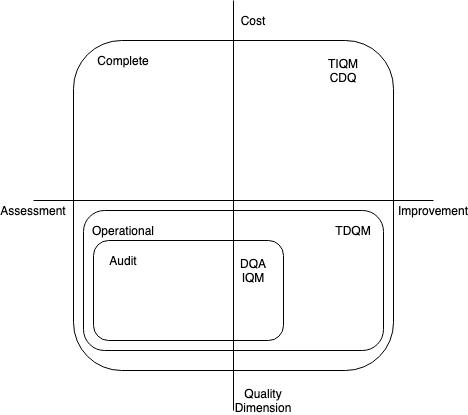
\includegraphics[width=0.75\textwidth]{Paper/figures/A classification of methodologies.png}
    \caption{A classification of methodologies.}
    \label{fig:classificationMethodologies}
  \end{figure}

\subsection{Summary of Methodologies}
We can classify these methodologies into 3 categories based on their emphasis on improvement, assessment, cost and quality dimensions. Figures \ref{fig:classificationMethodologies} show the methods positioned on a two-dimensional coordinated. The categories are:
(1) Complete methodologies, which provide support to both the assessment and improvement phases, and address both technical and economic issues;
(2) Audit methodologies, which focus on the assessment phase and provide limited support to the improvement phase;
(3) Operational methodologies, which focus on the technical issues of both the assessment and improvement phases, but do not address economic issues. (4) Economic methodologies, which focus on the evaluation of costs.

\begin{comment}
From a historical perspective, there exists a correlation between quality dimensions and the evolution of ICT technologies.
The evolution of information systems from monolithic to network-based has caused a growth of the number of data sources in both size and scope and, consequently has significantly increased the complexity of data quality management. DQ methodologies have started to focus on new quality dimensions, such as the completeness of the data source, the currency of data, and the consistency of the new data sources compared to the enterprise database. With the advent of the Web, data sources have become difficult to assess and control over time. At the same time, searching and navigating through the Web is potentially unlimited. As a consequence of this fast evolution, methodologies have started to address new quality dimensions, such as accessibility and reputation. Accessibility measures the ability of users to access data, given their culture, physical status and available technologies, and is important in cooperative and network-based information systems. Reputation (or trustworthiness) is a property of data sources measuring
\end{comment}
\subsubsection{Operational} focus DQ assessment on identifying the issues for which their improvement approach works best. One of the main contributions is the identification of a set of relevant dimensions to improve and the description of a few straightforward methods to assess them. For example, TDQM is a general-purpose methodology and suggests a complete set of relevant dimensions and improvement methods that can be applied in different contexts.
\subsubsection{Complete} are extremely helpful in providing a comprehensive frame- work to guide large DQ programs in organizations that process critical data and attribute to DQ a high strategic priority, such as banks and insurance companies. On the other hand, they show the classical trade-off between the applicability of the methodology and the lack of personalization to specific application domains or technological contexts. Being high-level and rather context independent, complete methodologies are only marginally affected by the evolution of ICT technologies and, over time have been revised to encompass the variety of data types, sources, and flows that are part of modern information systems.

\subsubsection{Audit} Most audit and improvement methodologies have a cost evaluation step. However, they mostly focus on the cost of DQ initiatives, while a complete cost-benefit analysis should also consider the cost of doing nothing, the cost of poor data quality, which is typically of an organizational nature. Economic methodologies,complement other methodologies and can be easily positioned within the overall framework provided by any complete methodology, focus on both aspects.

In CDQ, the overall evaluation of the cost of poor quality is further developed to take into account the fact that the same quality improvement can be obtained with different priorities and paths and the minimization of the cost of the data quality program is the main criterion to choose among alternative improvement processes.
The methodology suggests that different improvement processes can identified as paths of data- and process-driven techniques applied to the data bases, data flows and document bases involved in the improvement. Then, the costs of the different processes should be evaluated and compared, to select the minimum-cost process.
\begin{comment}

Experiences of use of early TDQM versions are reported in several U.S.A. Department of Defence (DoD) documents (see US Department of Defense [1994]). Specifically, the use of DQ tools developed over SQL scripts and programming approaches to check data quality are supported.
In Batini and Scannapieco [2006], a large-scale experience of the application of CDQ is reported, referring to the reorganization of Government to Business (G2B) relation- ships in Italy. The interactions with government are needed for several business events, such as starting a new business and evolving a business, which includes variations in legal status, board composition, senior management, and number of employees.
\end{comment}

\section{Conclusion}

This paper first introduces fundamentals of data quality, pipelines and classification of general assessment method, followed by the evaluation and analysis over five DQ assessment methods in term of different aspects.
Of all the surveyed methods, CDQ is considered to be the most complete, yet flexible, and simple to apply.
The completeness is achieved by considering existing techniques and tools and integrating them in a framework that can work in both intra- and inter-organizational contexts, and can be applied to all types of data, structured, semistructured and unstructured.
The methodology is flexible since it supports the user in the selection of the most suitable techniques and tools within each phase and in any context.
Experience suggests a “one size fits all” set of metrics is not a solution. The CDQ flexibility poses itself in great advantage over other methods.
Finally, CDQ is simple since it is organized in phases and each phase is characterized by a specific goal and set of techniques to apply.

The very motivation for this paper is to explore possibility of applying DQ assessment in academic research of software engineering, specifically CI/CD application. CI focuses on automation tools to allow development teams to integrate their efforts, build and test the code, while CD enables the code to be packaged and delivered with a fully automated deployment process. Both of the process are automated and generated logs and reports that are common in the format of semi-structured data, commonly stored in XML or HTML.
Therefore, the CDQ's capability of extension to other new metrics and flexibility make it the most suitable candidate for future application of DQ assessment in software engineering.

Two open issues are left to be investigated: DQ assessment method customized for specific information system and challenges in big data era.
From a historical perspective, there exists a correlation between quality dimensions and the evolution of ICT technologies.
The most critical issues with data quality management were error localization and correction in data sources, and record linkage between new data sources and preexisting data bases.
The evolution of information systems from monolithic to network-based has caused a growth of the number of data sources in both size and scope and, consequently has significantly increased the complexity of data quality management.

The characteristics of big data come down to the 4Vs: Volume, Velocity, Variety, and Value (Katal, Wazid, & Goudar, 2013). Volume refers to the tremendous volume of the data. Velocity means that data are being formed at an unprecedented speed and must be dealt with in a timely manner. Variety indicates that big data has all kinds of data types, and this diversity divides the data into structured data and unstructured data. These multityped data requires higher data processing capabilities.
Finally, Value represents low-value density. Value density is inversely proportional to total data size, the greater the big data scale, the less relatively valuable the data. Consequently, the cost of DQ assessment will gain significant importance is inevitable. How to accurately define and estimate the cost of DQ is another topic.

In the end, assessing data quality is an on-going effort that requires awareness of the fundamental principles underlying the development and context of application.

\bibliography{template}

\end{document}
